  %%%%%%%%%%%%%%%%%%%%%%%%%%%%%%%%%%%%%%%%%%%%%%%%%%%%%%%%%%%%%%%%%%%%%%
% LaTeX Example: Project Report

%%% Preamble
\documentclass[paper=a4, fontsize=11pt, abstract=on]{scrartcl}
\usepackage[T1]{fontenc}
\usepackage{fourier}
\usepackage{tabularx}
\usepackage[utf8]{inputenc}
\usepackage{hyperref}





\usepackage{listings}
\usepackage{color}

\definecolor{dkgreen}{rgb}{0,0.6,0}
\definecolor{gray}{rgb}{0.5,0.5,0.5}
\definecolor{mauve}{rgb}{0.58,0,0.82}
\lstset{frame=tb,
  language=[Visual]C++,
  aboveskip=3mm,
  belowskip=3mm,
  showstringspaces=false,
  columns=flexible,
  basicstyle={\small\ttfamily},
  numbers=none,
  numberstyle=\tiny\color{gray},
  keywordstyle=\color{blue},
  commentstyle=\color{dkgreen},
  stringstyle=\color{mauve},
  breaklines=true,
  breakatwhitespace=true,
  tabsize=3
}
\usepackage{graphicx}
\usepackage{caption}
\usepackage{subcaption}

\usepackage[english]{babel}															% English language/hyphenation
\usepackage[protrusion=true,expansion=true]{microtype}	
\usepackage{amsmath,amsfonts,amsthm} % Math packages

\usepackage{url}
%\usepackage[hang, small,labelfont=bf,up,textfont=it,up]{caption}


%%% Custom sectioning
\usepackage{sectsty}
\allsectionsfont{\normalfont\scshape}
\usepackage{float}
\usepackage{amsmath}
\usepackage{mathtools}
\usepackage{ragged2e}

\usepackage{nomencl}
\makenomenclature

%%% Custom headers/footers (fancyhdr package)
\usepackage{fancyhdr}
\pagestyle{fancyplain}
\fancyhead{}											% No page header
\fancyfoot[L]{}											% Empty 
\fancyfoot[C]{}											% Empty
\fancyfoot[R]{\thepage}									% Pagenumbering
\renewcommand{\headrulewidth}{0pt}			% Remove header underlines
\renewcommand{\footrulewidth}{0pt}				% Remove footer underlines
\setlength{\headheight}{13.6pt}
   \renewcommand*\abstractname{Summary}

%%% Equation and float numbering
\numberwithin{equation}{section}		% Equationnumbering: section.eq#
\numberwithin{figure}{section}			% Figurenumbering: section.fig#
\numberwithin{table}{section}				% Tablenumbering: section.tab#


%%% Maketitle metadata

\newcommand{\horrule}[1]{\rule{\linewidth}{#1}} 	% Horizontal rule

\title{
		%\vspace{-1in} 	
		\usefont{OT1}{bch}{b}{n}
		\normalfont \normalsize \textsc{} \\ [25pt]
		
\includegraphics[width=0.3\linewidth]{ubc.png} \\
		%
\includegraphics[width=0.4\linewidth]{tru}		
		\horrule{0.5pt} \\[0.2cm]
		\huge Lab \#1 : Portable Non-invasive Measurement of Drag Coefficients  \\
		\horrule{2pt} \\[0.005cm]
}
\author{
		\normalfont 								\normalsize
        Jerin Roberts\\[-5pt]		\normalsize
        \today
}
\date{}




%%% Begin document
\begin{document}
\maketitle
\begin{center}
\begin{tabular}{l r}


Supervisor: & Dr. Patrick Kirchen  \\ % supervisor
Locations: & University of British Columbia


\end{tabular}
\end{center}
\newpage
\begin{abstract}
Measuring the coefficient of drag precisely usually requires a setup which sets an invasive constraint on the object in question. In this experiment we set out to test a method for non-invasive measurement of the drag coefficient for two common sports objects. The method employs object tracking software to calculated the drag coefficient as the object falls to the ground. The average drag coefficients for the shuttlecock and the table tennis ball were found to be 0.949$\pm$0.438 and 0.522$\pm$0.382 respectively. The viability of the method was tested and found to be accurate compared to external sources. Such a technique could have application in the sports industry provided the precision is improved which will require further research and significant error reduction.
\end{abstract}


\newpage
\tableofcontents
\listoffigures
\listoftables
\newpage
\lstset{language=[Visual]C++}
\section{Introduction}



 The force of drag is studied in many engineering fields such as aerodynamics, fluid mechanics and thermal-fluids. Understanding the effects of drag and minimizing its effect can vastly improve performance and efficiency for many systems. For professional sports characterizing the effect of drag on regulation equipment is crucial task. In order for players to compete on equal grounds the sport equipment they use needs to be held to a specific standard. Defining the drag characteristics of a sports ball is one standard that can help keep the game competitive and fair. This is especially critical for sports where drag and lift forces play a key roll in game-play dynamics. Measuring the coefficient of drag precisely usually requires a setup which sets an invasive constraint on the object in question. In this experiment we set out to test a method for non-invasive measurement of the drag coefficient for two common sports objects. Such a technique could have application in the sports industry and could provide a fast portable method for determining if sports objects are within aerodynamic regulation.

\section{Background}
\mbox{}% need to run this: makeindex Lab1.nlo -s nomencl.ist -o Lab1.nls

 
\nomenclature{$g$}{Acceleration due to Gravity in a Vacuum $m/s^2$}
\nomenclature{$\rho$}{Density $kg/m^3$}
\nomenclature{$C_D$}{Drag Coefficient}
\nomenclature{$Re$}{Reynolds Number}
\nomenclature{$A$}{Cross-Sectional Projected Area $m^2$}
\nomenclature{$v$}{Velocity $m/s$}
\nomenclature{$m$}{Mass $kg$}
\nomenclature{$\mu$}{Dynamic Viscosity $Pa-s$}
\nomenclature{$L$}{Characteristic Linear Dimension $m$}
 
\printnomenclature
\subsection{Theory}
Any object that travels through a fluid will experience an opposing drag force which is related to the objects shape. Drag is generally the result of frictional and viscous forces between the object and fluid. The general expression for force on an object experience due to drag for high velocities is displayed as equation \ref{drag}.
 \begin{equation}
\label{drag}
F_D= \frac{1}{2}\rho v^2C_DA
\end{equation}

\begin{equation}
\label{grav}
F_g= mg = 9.806 m/s^2
\end{equation}

The term $C_D$ is known as the drag coefficient (dimensionless parameter), $F_D$ is the drag force, $\rho$ is the density of the fluid, $v$ is the speed of the object relative to the fluid, and $A$ is the cross sectional area. For this experiment we are considering the two major forces acting on the sports object as they fall to the ground; gravity ($F_g$) and drag ($F_D$). These forces are opposing therefore the measured force will be the sum of gravity and drag as shown in equation \ref{force}

\begin{equation}
\label{force}
\vec{F}_{object}= \sum{}{}\vec{F}_i = (F_D-F_g) \hat{k}
\end{equation}


\subsection{Measurement}
The are many methods for measuring the drag ceofficent of an object. One of the most common ways is to attach the object to a lift balance in closed wind tunnel. This method ensures the flow is well defined and enables sensitive measurements of drag force for a wide range of flows\cite{p0}. However this method is not portable and requires fastening the sport object to a sensor or load cell. Another method for measurement is using a laser to measure the object as it falls through a volume of fluid. This method can also provide details regarding the objects terminal velocity and drag effects for low velocity. However this method again lacks portability as it requires the object to cross a set of laser beams while sinking in a fluid vessel\cite{p1}. In this experiment we plan to test the viability of applying tracking software for portable non-invasive drag coefficient analysis.

\section{Methodology}

\subsection{Overview}
In order to measure drag we first needed a method to measure the motion of an object falling through the air. By knowing the position of the object relative to time, one will also know the velocity and subsequently the acceleration of the object. The acceleration can be compared to what would be expected if the object were falling in a vacuum, for which any discrepancy between the two will assumed to be caused by drag. The measurement of drag force was found using a video capturing device. Two objects were dropped dropped from varying heights and recorded by a video camera capturing the trajectory to the ground in order to compared the effects of drag. 


  
\subsection{Procedure}
A GoPro hero 1 camera with a 60fps frame rate was setup a known distance from the screen as shown in figure \ref{schem}. For each run the camera record the flight of the object being dropped. A regulation table tennis ball and a regulation badminton shuttlecock were each dropped 20 times in front of the screen from varying heights and recorded as they fell through the tracking zone. A tracking zone was used in order to reduce the uncertainties associated with the fish-eye lens of the camera as the effect of the lens was not well characterized. Both the masses and the diameters of the sports objects were measured and recorded.

\begin{figure}[H]
\centering
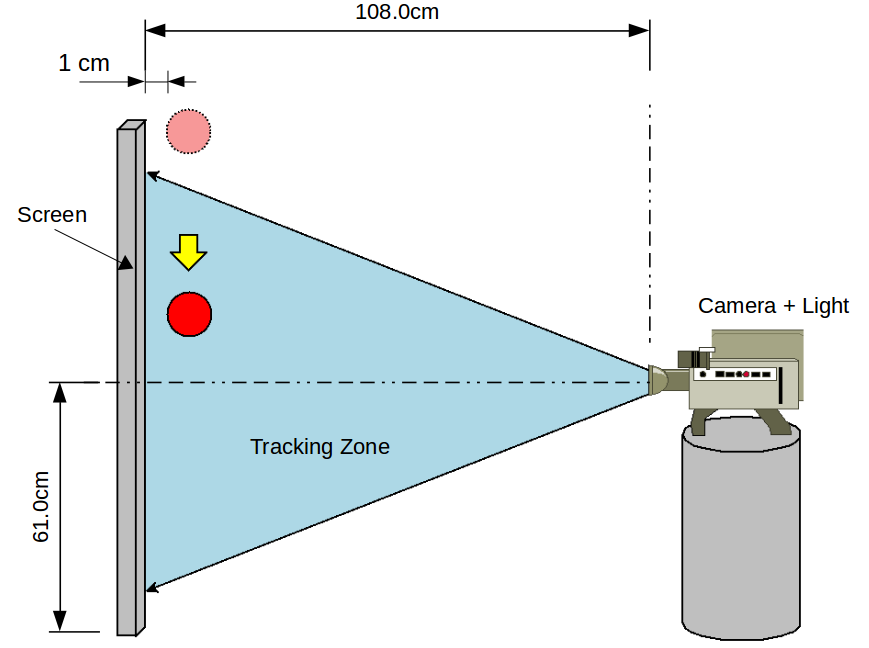
\includegraphics[width=0.75\linewidth]{schem}
\caption{Simplified experimental apparatus}
\label{schem}
\end{figure}

\begin{figure}[H]
\centering
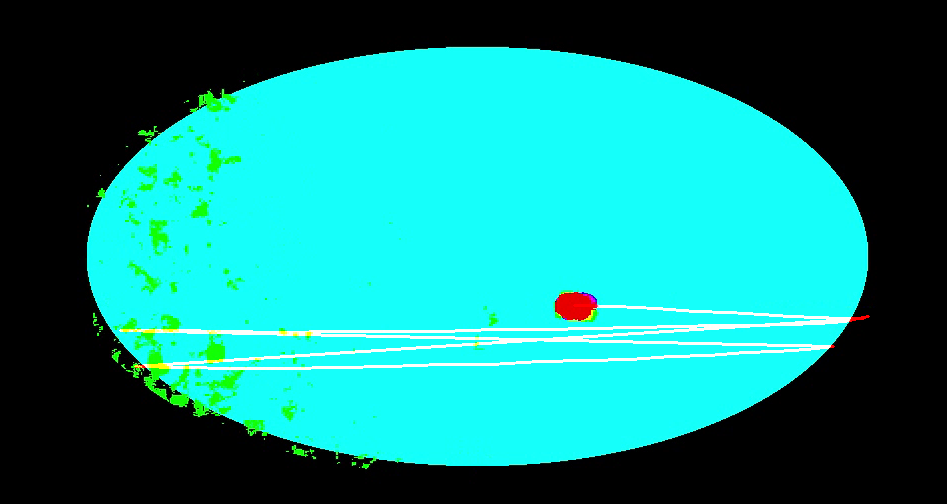
\includegraphics[width=0.5\linewidth]{contrast.jpg}
\caption{A sample output of the openCV program, where the object being tracked is contrasted in red as it falls right to left. Lines are drawn indicating the object is being tracked}
\label{cont}
\end{figure}




\subsection{Object Tracking}
In order to measure the distance traveled for each frame, an object tracking program (Appendix A.1) was written making use openCV libraries. The program would track objects of a specified color. For this experiment objects were painted red and allowed to fall in front of a white background greatly contrasting the object. The program filters all colors except for the one specified. Additionally contrasting, brightness and vignette filters were applied to the original video file in order to emphasize the color of the falling object while filtering out undesirable hues present in the background. 

\begin{figure}[H]
\centering
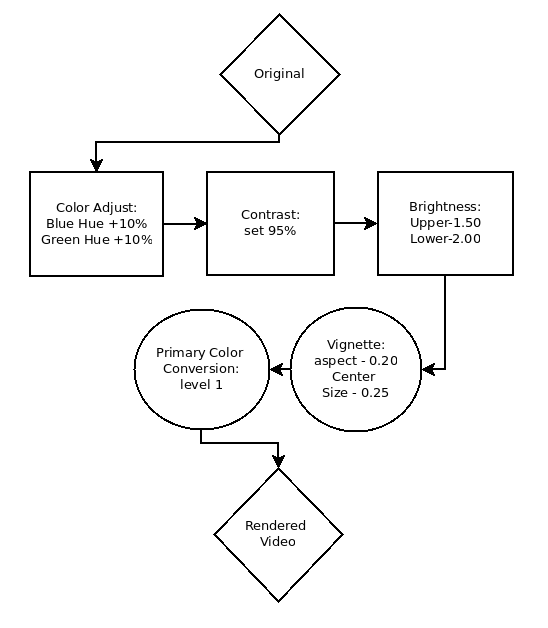
\includegraphics[width=0.6\linewidth]{rend}
\caption{Process schematic for video modification using OpenShot video editor}
\label{rend}
\end{figure}

A process schematic for external video rendering is shown in figure \ref{rend} and example of a filtered frame is displayed in figure \ref{cont}. From here the area and moments that the color occupies are calculated. Using this the program finds the centroid of the contrasted color. If only a large object is detected (beyond noise) a center point of the detected area is recorded for each frame. The program iterates through all frames providing pixel coordinates for the object being tracked. These coordinates are then converted using a calibration constant. 

\subsection{Calibration}
Calibration was needed to convert pixel coordinates into distance displace by the falling object. Eight small red dots were attached to the white backdrop at $0.03m$ increments. Each dot was recorded individually and its pixel coordinate calculated. The cameras position remained unaltered between recordings. 
\begin{table}[H]
\begin{center}
    \begin{tabular}{ | p{0.25\linewidth} | p{0.25\linewidth} | p{0.15\linewidth}|}
 \hline  
     \RaggedRight \textbf{Pixel Coordinate (x)}
    &\RaggedRight \textbf{Difference (x2-x1)}
    &\RaggedRight \textbf{Average} 
    \\ \hline  
           \RaggedRight 954.41 
    &\RaggedRight n/a
    &\RaggedRight  
    \\ \hline 
           \RaggedRight 985.95
    &\RaggedRight 31.54
    &\RaggedRight 
    \\ \hline 
           \RaggedRight 1016.6 
    &\RaggedRight 30.65
    &\RaggedRight  
    \\ \hline 
           \RaggedRight 1074.46
    &\RaggedRight 29.63
    &\RaggedRight 
    \\ \hline 
           \RaggedRight 1102.13 
    &\RaggedRight 27.67
    &\RaggedRight  
    \\ \hline 
           \RaggedRight 1129.41 
    &\RaggedRight 27.28
    &\RaggedRight 
    \\ \hline 
      \RaggedRight 1153.72 
    &\RaggedRight 24.30
    &\RaggedRight 0.03m per $28.47 \pm 2.64$
    \\ \hline 
    
    
    \end{tabular}
\end{center} 
\caption{Sample data used for calibration constant}
\label{cali} 
\end{table}
 The distance found between each dot was averaged and used as the calibration constant. The pixel data recorded for calibration is displayed in table \ref{cali} 
The Calibration constant was found to be 1.05$*10^{-3}\pm$ 9.7$*10^{-5}$.
\subsection{Calculations}

\begin{table}[H]
\begin{center}
    \begin{tabular}{ | p{0.3\linewidth} | p{0.15\linewidth} | p{0.25\linewidth}|}
 \hline  
     \RaggedRight \textbf{Sports Object}
    &\RaggedRight \textbf{mass (g)}
    &\RaggedRight \textbf{Area ($m^2$)} 
    \\ \hline  
       \RaggedRight Badminton Shuttlecock 
    &\RaggedRight 3.51$\pm$0.05
    &\RaggedRight 0.002827$\pm$0.00014 
    \\ \hline 
           \RaggedRight Table Tennis Ball
    &\RaggedRight 2.73$\pm$0.05
    &\RaggedRight 0.001256$\pm$0.00006 
    \\ \hline 
   
    \end{tabular}
\end{center} 
\caption{Specifications of sports objects}
\label{spec} 
\end{table}
In order to calculate the drag coefficient we needed to find the force acting on the object due to drag. Since we knew the conventional rate at which an object accelerates in a vacuum, the de-acceleration due to drag could be known by indirectly measuring the sports balls acceleration (equation \ref{drag2}).

\begin{equation}
\label{drag2}
F_D = m(a_g-a_{object})
\end{equation}


\begin{equation}
\label{poly2}
d= At^2+Bt+C
\end{equation}


 


Position with respect to time (framerate) was measured and recorded. In order to reduce error amplification a 2nd order polynomial fit, listed as equation \ref{poly2}, was applied for each data set where $A,B$ and $C$ are the fit parameters. An expression for the average acceleration was calculated by taking the second derivative of the fit function for distance with respect to time (ie $a = 2A$). The average acceleration for the sports object was referenced against the acceleration due to gravity (vacuum) in order to calculate a value for the force of drag. 
 
\begin{equation}
\label{reynolds}
Re= \frac{\rho vL}{\mu}
\end{equation} 
 
Using the function for velocity ($v = At+B$) and the Force of drag $F_D$, the drag coefficient $C_D$ was calculated using equation \ref{drag} and data from table \ref{spec}. The drag coefficients calculated for all 20 runs were then plotted as a function of velocity in the form of Reynolds number $Re$ calculated using equation \ref{reynolds}. Coefficients found to be less than zero were ignored as this implies faster than gravity acceleration. The error for the calculation was computed by incrementally taking slices for Reynolds numbers and finding the standard deviation of the drag coefficients in that slice. The Standard deviation is then plotted as a function of Reynolds number $Re$.
 
 
 
   
\section{Results}
\subsection{Overview}


\begin{figure}[H]
        \centering
        \begin{subfigure}[H]{0.45\textwidth}
                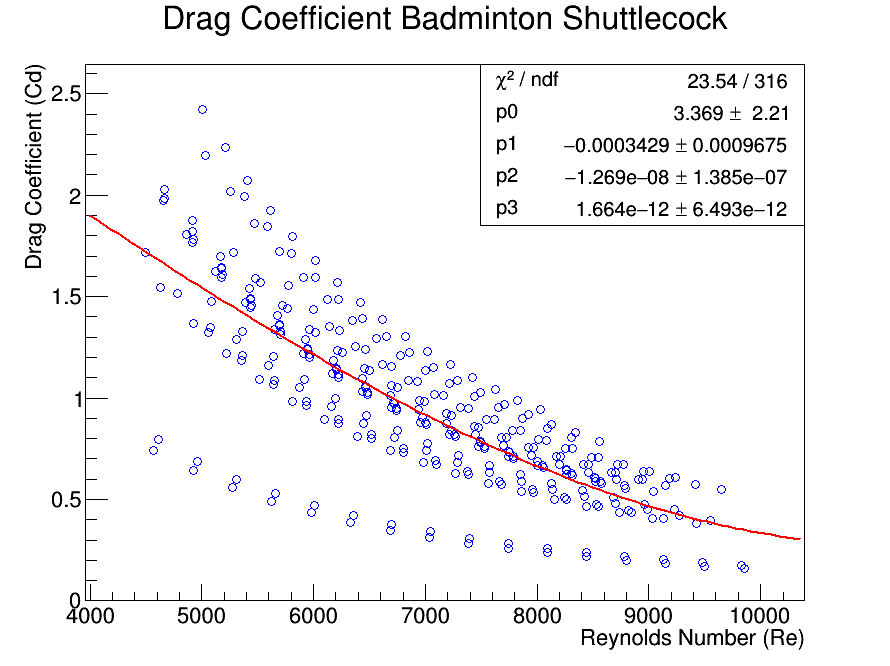
\includegraphics[width = 7.5cm]{shut}
                \caption{}
				
        \end{subfigure}%
       ~~~~~
        \begin{subfigure}[h]{0.45\textwidth}
                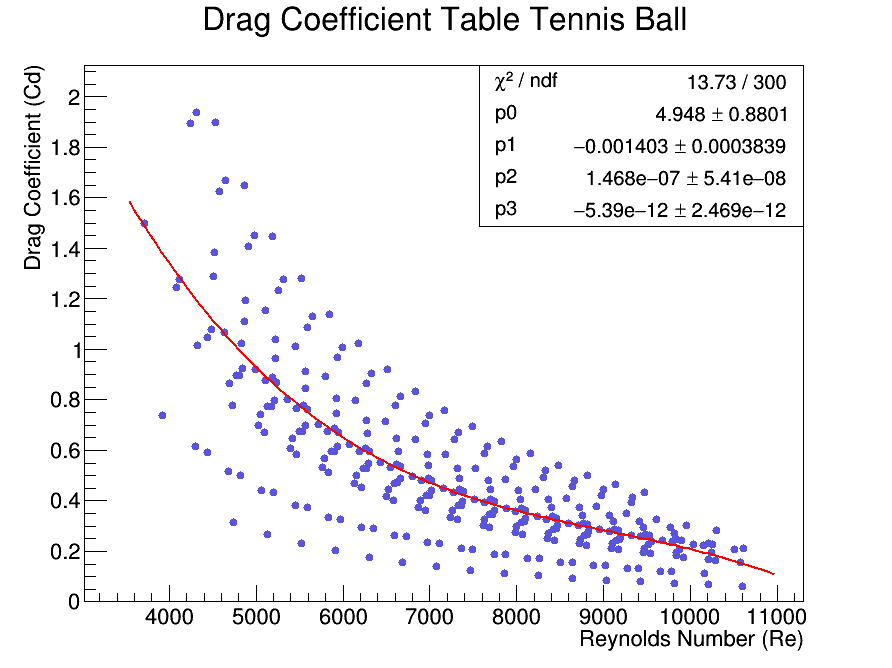
\includegraphics[width = 7.5cm]{ping}
                \caption{}
                
        \end{subfigure}
        ~~~~~
        \begin{subfigure}[h]{0.45\textwidth}
                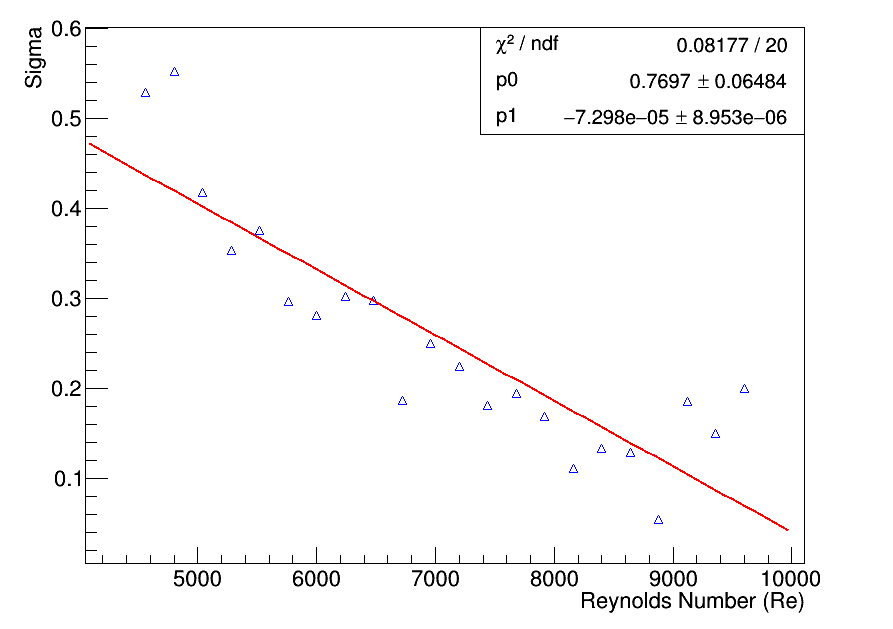
\includegraphics[width = 7.5cm]{shutst}
                \caption{}               
        \end{subfigure}
        ~~~~~
        \begin{subfigure}[h]{0.45\textwidth}
                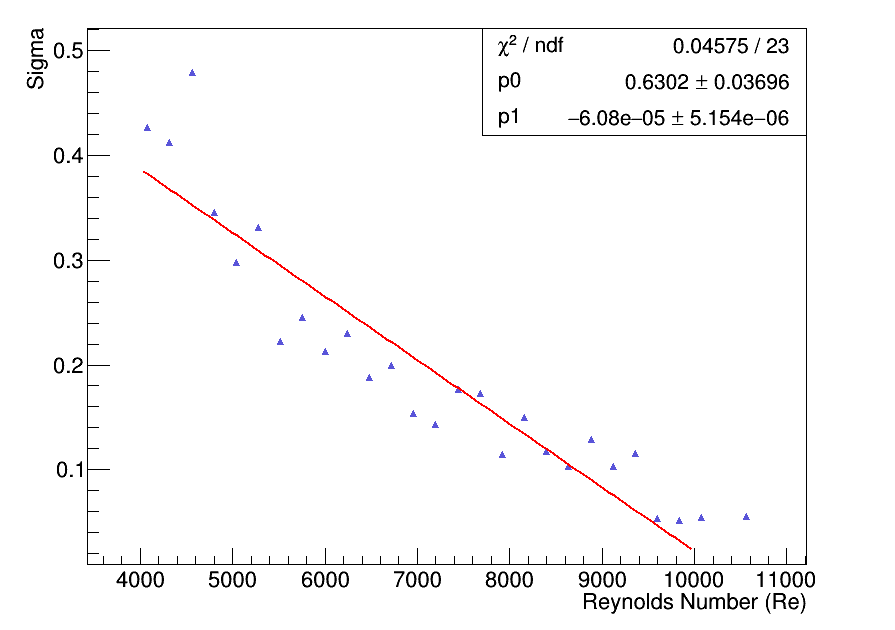
\includegraphics[width = 7.5cm]{pingst}
                \caption{}                
        \end{subfigure}
        \caption{Drag Coefficient as a function of Reynolds (Top) and Standard Deviation as function of Reynolds (Bottom)}
        \label{results}
\end{figure}
 The drag coefficients of a Badminton Shuttlecock and a Table Tennis Ball were measured for varying velocities and plotted as a function of Reynolds number. Figure \ref{results} displays the results of the experiment. Generally the drag coefficient is expressed as an average over measured Reynolds numbers. Figure \ref{hist} displays the average $C_D$ for both the shuttlecock and the table tennis ball. The average drag coefficient for the shuttlecock and the table tennis ball was found to be 0.949$\pm$0.438 and 0.522$\pm$0.382 respectively. The average drag coefficient value for a Badminton shuttlecock can vary among studies. Its often found in a range of $C_D$ values from 0.50 to 0.75 for similar Reynolds number range $10^4-10^5$ \cite{p1}. Additionally the table tennis ball or spherical object has be known to have $C_D$ values ranging from 0.40 to 0.55 for a Reynolds range of $10^3-10^4$ \cite{p2}. The accuracy of the measured values fall well within these ranges and agree well with current experimental studies. However the precision of the experiment is not within acceptable limits. The size of the standard deviation for slices of Reynolds shows the error of the method is very large (40-50\%) . We expect some variance over large Reynolds regions however for small slices this should have be reduced. Based on this method the real value could be found outside standard or well known ranges. 

\begin{figure}[H]
        \centering
        \begin{subfigure}[h]{0.5\textwidth}
                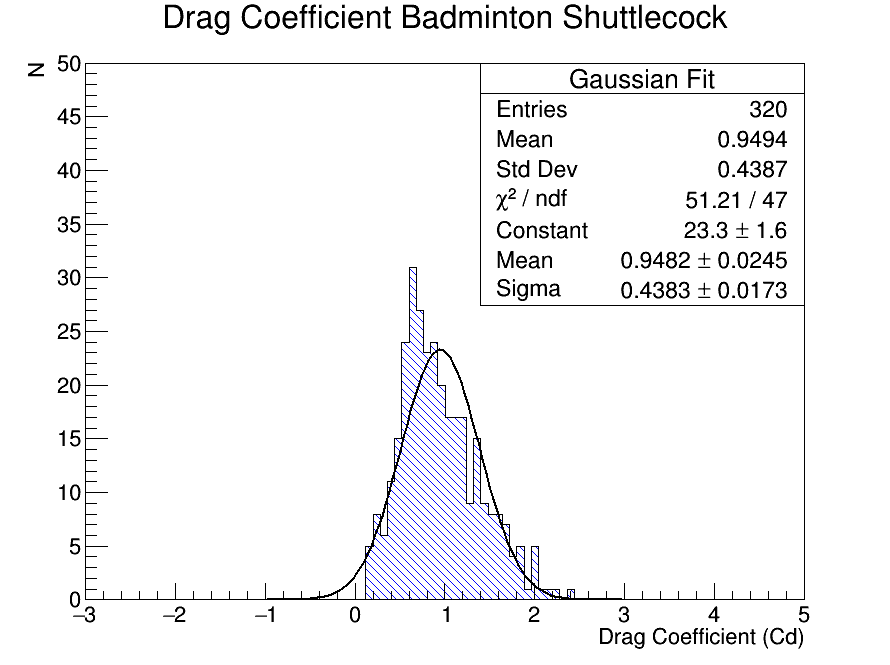
\includegraphics[width = 8cm]{hists}
                \caption{}
				
        \end{subfigure}%
       ~~~~~
        \begin{subfigure}[h]{0.5\textwidth}
                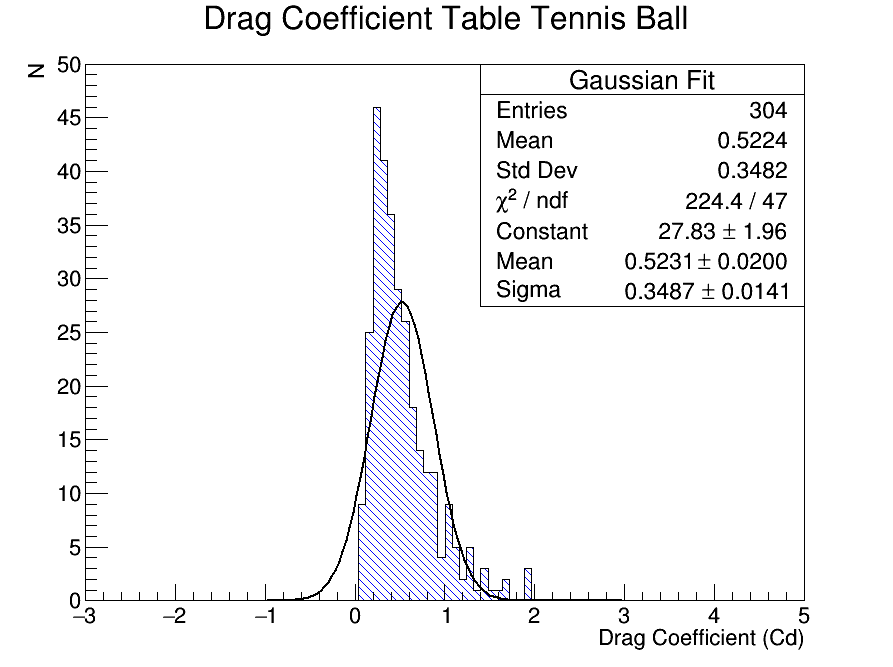
\includegraphics[width = 8cm]{histp}
                \caption{}
                
        \end{subfigure}
        \caption{Average Drag Coefficient}
        \label{hist}
\end{figure}

\subsection{Sources of Error}

The are several sources of error that contribute to this problem. This first is the nature of measurement method. Since the drag force is not directly measured we need to infer it by taking two derivatives of the function for measured distance. Any Error found in the distance measurement will be inherently amplified in the drag force calculation. Unfortunately there is no (simple) non-invasive way to measure force. Fitting the displacement function can help this problem but ultimately reduces information known about the system. Therefore the improvements need to made to the displacement measurement itself. The method of calculating trajectory points based on the centroid of the contrasted area can also cause significant error. As the object moves relative to the light source its glare changes distorting the final shape of the detected area as white objects are not detected. This ultimately causes undesirable shifts to the calculated center point of the tracked area. Using uniform matte colored object and smarter lighting conditions could be used to reduce this error for future tests. Improvements to the video recording system will likely reduce sources of error. The camera used in the experiment had an above average frame rate, however in majority of the frames the objects outline was skewed which causes a shifted center point. This normally indicates the frame rate is too low or the exposure time too great for the speed of the object. A higher resolution camera with a faster capture time formatted for high speed objects would help reduce the errors found in the displacement measurements. Additionally the use of a fish-eye lens was likely a source or error. For future measurements the effect of the lens relative to interpreted displacement should be fully characterized in order to apply a corrective transformation. 
\section{Conclusion}
In this experiment we set out to test a method for non-invasive measurement of the drag coefficient for two common sports objects. We were able test the viability of the method and found it to be accurate compared to external sources. Unfortunately the precision of the method is very poor. Such a technique could have application in the sports industry provided the precision is improved which will require further research. Ultimately based on this analysis this method would provide a poor means for determining the aerodynamic standards on sports equipment. With the majority of source error residing in the software implemented tracking which is the one aspect that makes this method unique, its unlikely this setup would be suitable for sports related standards policing. 









\appendix
\section{Appendix} \label{App:Appendix}
\subsection{openCV object tracking script}
\begin{lstlisting}
#include <iostream>
#include <fstream> //printf
#include <unistd.h>  //usleep
#include "opencv2/highgui/highgui.hpp"
#include "opencv2/imgproc/imgproc.hpp"
#include <vector>

using namespace cv;
using namespace std;

struct sel{
float xpos;
float ypos;
float time;

};

struct obj{
vector<sel> eframes;
};

void write_data(string & datafile, obj myset);

 int main( int argc, char** argv )
 { 
  string myfile = "tmp";	 
  obj myset;
 
    VideoCapture cap("video/ping1.mp4"); //video from file

    if ( !cap.isOpened() )  // if fails
    {
         cout << "Cannot open the web cam" << endl;
         return -1;
    }

    namedWindow("Control", CV_WINDOW_AUTOSIZE); //create a window

 int iLowH = 0;
 int iHighH = 179;
 int iLowS = 255; 
 int iHighS = 255;
 int iLowV = 189;
 int iHighV = 255;

 //Create trackbars in "Control" window
 createTrackbar("LowH", "Control", &iLowH, 179); //Hue (0 - 179)
 createTrackbar("HighH", "Control", &iHighH, 179);
 createTrackbar("LowS", "Control", &iLowS, 255); //Saturation (0 - 255)
 createTrackbar("HighS", "Control", &iHighS, 255);
 createTrackbar("LowV", "Control", &iLowV, 255);//Value (0 - 255)
 createTrackbar("HighV", "Control", &iHighV, 255);

float iLastX = -1; 
float iLastY = -1;

 //Capture a temporary image from the camera
 Mat imgTmp;
 cap.read(imgTmp); 

 //Create a black image with the size as the camera output
 Mat imgLines = Mat::zeros( imgTmp.size(), CV_8UC3 );;
 int frame = 0;

    while (true)
    {   //usleep(100000);
    	++frame;
        Mat imgOriginal;
        bool bSuccess = cap.read(imgOriginal); // read a new frame from video

         if (!bSuccess) 
        {    cout << "Cannot read a frame from video stream" << endl;
             break;
        }

  Mat imgHSV;
  cvtColor(imgOriginal, imgHSV, COLOR_BGR2HSV); //Convert the captured frame from BGR to HSV 
  Mat imgThresholded;
  inRange(imgHSV, Scalar(iLowH, iLowS, iLowV), Scalar(iHighH, iHighS, iHighV), imgThresholded); //Threshold the image
      
  //removes small objects from the foreground
  erode(imgThresholded, imgThresholded, getStructuringElement(MORPH_ELLIPSE, Size(5, 5)) );
  dilate( imgThresholded, imgThresholded, getStructuringElement(MORPH_ELLIPSE, Size(5, 5)) ); 

  //remove small holes from the foreground
  dilate( imgThresholded, imgThresholded, getStructuringElement(MORPH_ELLIPSE, Size(5, 5)) ); 
  erode(imgThresholded, imgThresholded, getStructuringElement(MORPH_ELLIPSE, Size(5, 5)) );

  //Calculate the moments of the thresholded image
  Moments oMoments = moments(imgThresholded);

  double dM01 = oMoments.m01;
  double dM10 = oMoments.m10;
  double dArea = oMoments.m00;
  float posX = 0;
  float posY = 0;
  float vX = 0;
  float vY = 0;
  
  // if the area <= 1000, rest is noise
  if (dArea > 1000)
  {
   //calculate the position of the ball
   sel temppoint;   
   posX = dM10 / dArea;
   posY = dM01 / dArea;
    temppoint.xpos = posX;
    temppoint.ypos = posY;
    temppoint.time = frame;
    
    printf("Xpos: %f  Ypos: %f frame: %d\n", posX, posY, frame); 
    
   myset.eframes.push_back(temppoint);                       
   if (iLastX >= 0 && iLastY >= 0 && posX >= 0 && posY >= 0)
   {
    //Draw a red line from the previous point to the current point
    line(imgLines, Point(posX, posY), Point(iLastX, iLastY), Scalar(0,0,255), 2);
   }
   iLastX = posX;
   iLastY = posY;
  }

  imshow("Thresholded Image", imgThresholded); //show the thresholded image

  imgOriginal = imgOriginal + imgLines;
  imshow("Original", imgOriginal); //show the original image

        if (waitKey(30) == 27) //wait for 'esc' key press for 30ms. If 'esc' key is pressed, break loop
       {
            cout << "esc key is pressed by user" << endl;
            break; 
       }
    }       
   write_data(myfile, myset);
   return 0;
}


void write_data(string & datafile, obj myset)
{
sel temp;
std::ofstream myfile;
datafile.append(".txt");
const char * c;
c = datafile.c_str();
myfile.open(c,fstream::out);

   for(int i = 0; i < myset.eframes.size(); ++i)
    {
    sel temp;
    temp = myset.eframes.at(i);    
    float posX = temp.xpos;
    float posY = temp.ypos;
    float frame = temp.time;    
    myfile << "data " << posX << " " << posY << " " << frame << "\n";
    printf("writing Xpos: %f  Ypos: %f frame: %f\n", posX, posY, frame); 
    }
  myfile.close();

}


\end{lstlisting}


\begin{thebibliography}{99} % Beamer does not support BibTeX so references must be inserted manually as below
\bibitem[Galam, 2009]{p0}Firoz Alam, Harun Chowdhury,C.Theppadungporn and Aleksandar Subic  (2009)
\newblock "A study of Badminton shuttlecock aerodynamics",  RMIT University


\bibitem[Cooke, 1999]{p1} Alison J. Cooke (1999)
\newblock "Shuttlecock Aerodynamics", Department of Engineering, Cambridge University


\bibitem[Cimbala, 2012]{p2} J.M. Cimbala (1999)
\newblock "Drag on Spheres", Department of Engineering, Penn State Univeristy
\end{thebibliography}


%%% End document
\end{document}